% Options for packages loaded elsewhere
% Options for packages loaded elsewhere
\PassOptionsToPackage{unicode}{hyperref}
\PassOptionsToPackage{hyphens}{url}
\PassOptionsToPackage{dvipsnames,svgnames,x11names}{xcolor}
%
\documentclass[
  a4paper,
  DIV=11,
  numbers=noendperiod]{scrartcl}
\usepackage{xcolor}
\usepackage{amsmath,amssymb}
\setcounter{secnumdepth}{-\maxdimen} % remove section numbering
\usepackage{iftex}
\ifPDFTeX
  \usepackage[T1]{fontenc}
  \usepackage[utf8]{inputenc}
  \usepackage{textcomp} % provide euro and other symbols
\else % if luatex or xetex
  \usepackage{unicode-math} % this also loads fontspec
  \defaultfontfeatures{Scale=MatchLowercase}
  \defaultfontfeatures[\rmfamily]{Ligatures=TeX,Scale=1}
\fi
\usepackage{lmodern}
\ifPDFTeX\else
  % xetex/luatex font selection
\fi
% Use upquote if available, for straight quotes in verbatim environments
\IfFileExists{upquote.sty}{\usepackage{upquote}}{}
\IfFileExists{microtype.sty}{% use microtype if available
  \usepackage[]{microtype}
  \UseMicrotypeSet[protrusion]{basicmath} % disable protrusion for tt fonts
}{}
\makeatletter
\@ifundefined{KOMAClassName}{% if non-KOMA class
  \IfFileExists{parskip.sty}{%
    \usepackage{parskip}
  }{% else
    \setlength{\parindent}{0pt}
    \setlength{\parskip}{6pt plus 2pt minus 1pt}}
}{% if KOMA class
  \KOMAoptions{parskip=half}}
\makeatother
% Make \paragraph and \subparagraph free-standing
\makeatletter
\ifx\paragraph\undefined\else
  \let\oldparagraph\paragraph
  \renewcommand{\paragraph}{
    \@ifstar
      \xxxParagraphStar
      \xxxParagraphNoStar
  }
  \newcommand{\xxxParagraphStar}[1]{\oldparagraph*{#1}\mbox{}}
  \newcommand{\xxxParagraphNoStar}[1]{\oldparagraph{#1}\mbox{}}
\fi
\ifx\subparagraph\undefined\else
  \let\oldsubparagraph\subparagraph
  \renewcommand{\subparagraph}{
    \@ifstar
      \xxxSubParagraphStar
      \xxxSubParagraphNoStar
  }
  \newcommand{\xxxSubParagraphStar}[1]{\oldsubparagraph*{#1}\mbox{}}
  \newcommand{\xxxSubParagraphNoStar}[1]{\oldsubparagraph{#1}\mbox{}}
\fi
\makeatother

\usepackage{color}
\usepackage{fancyvrb}
\newcommand{\VerbBar}{|}
\newcommand{\VERB}{\Verb[commandchars=\\\{\}]}
\DefineVerbatimEnvironment{Highlighting}{Verbatim}{commandchars=\\\{\}}
% Add ',fontsize=\small' for more characters per line
\usepackage{framed}
\definecolor{shadecolor}{RGB}{241,243,245}
\newenvironment{Shaded}{\begin{snugshade}}{\end{snugshade}}
\newcommand{\AlertTok}[1]{\textcolor[rgb]{0.68,0.00,0.00}{#1}}
\newcommand{\AnnotationTok}[1]{\textcolor[rgb]{0.37,0.37,0.37}{#1}}
\newcommand{\AttributeTok}[1]{\textcolor[rgb]{0.40,0.45,0.13}{#1}}
\newcommand{\BaseNTok}[1]{\textcolor[rgb]{0.68,0.00,0.00}{#1}}
\newcommand{\BuiltInTok}[1]{\textcolor[rgb]{0.00,0.23,0.31}{#1}}
\newcommand{\CharTok}[1]{\textcolor[rgb]{0.13,0.47,0.30}{#1}}
\newcommand{\CommentTok}[1]{\textcolor[rgb]{0.37,0.37,0.37}{#1}}
\newcommand{\CommentVarTok}[1]{\textcolor[rgb]{0.37,0.37,0.37}{\textit{#1}}}
\newcommand{\ConstantTok}[1]{\textcolor[rgb]{0.56,0.35,0.01}{#1}}
\newcommand{\ControlFlowTok}[1]{\textcolor[rgb]{0.00,0.23,0.31}{\textbf{#1}}}
\newcommand{\DataTypeTok}[1]{\textcolor[rgb]{0.68,0.00,0.00}{#1}}
\newcommand{\DecValTok}[1]{\textcolor[rgb]{0.68,0.00,0.00}{#1}}
\newcommand{\DocumentationTok}[1]{\textcolor[rgb]{0.37,0.37,0.37}{\textit{#1}}}
\newcommand{\ErrorTok}[1]{\textcolor[rgb]{0.68,0.00,0.00}{#1}}
\newcommand{\ExtensionTok}[1]{\textcolor[rgb]{0.00,0.23,0.31}{#1}}
\newcommand{\FloatTok}[1]{\textcolor[rgb]{0.68,0.00,0.00}{#1}}
\newcommand{\FunctionTok}[1]{\textcolor[rgb]{0.28,0.35,0.67}{#1}}
\newcommand{\ImportTok}[1]{\textcolor[rgb]{0.00,0.46,0.62}{#1}}
\newcommand{\InformationTok}[1]{\textcolor[rgb]{0.37,0.37,0.37}{#1}}
\newcommand{\KeywordTok}[1]{\textcolor[rgb]{0.00,0.23,0.31}{\textbf{#1}}}
\newcommand{\NormalTok}[1]{\textcolor[rgb]{0.00,0.23,0.31}{#1}}
\newcommand{\OperatorTok}[1]{\textcolor[rgb]{0.37,0.37,0.37}{#1}}
\newcommand{\OtherTok}[1]{\textcolor[rgb]{0.00,0.23,0.31}{#1}}
\newcommand{\PreprocessorTok}[1]{\textcolor[rgb]{0.68,0.00,0.00}{#1}}
\newcommand{\RegionMarkerTok}[1]{\textcolor[rgb]{0.00,0.23,0.31}{#1}}
\newcommand{\SpecialCharTok}[1]{\textcolor[rgb]{0.37,0.37,0.37}{#1}}
\newcommand{\SpecialStringTok}[1]{\textcolor[rgb]{0.13,0.47,0.30}{#1}}
\newcommand{\StringTok}[1]{\textcolor[rgb]{0.13,0.47,0.30}{#1}}
\newcommand{\VariableTok}[1]{\textcolor[rgb]{0.07,0.07,0.07}{#1}}
\newcommand{\VerbatimStringTok}[1]{\textcolor[rgb]{0.13,0.47,0.30}{#1}}
\newcommand{\WarningTok}[1]{\textcolor[rgb]{0.37,0.37,0.37}{\textit{#1}}}

\usepackage{longtable,booktabs,array}
\newcounter{none} % for unnumbered tables
\usepackage{calc} % for calculating minipage widths
% Correct order of tables after \paragraph or \subparagraph
\usepackage{etoolbox}
\makeatletter
\patchcmd\longtable{\par}{\if@noskipsec\mbox{}\fi\par}{}{}
\makeatother
% Allow footnotes in longtable head/foot
\IfFileExists{footnotehyper.sty}{\usepackage{footnotehyper}}{\usepackage{footnote}}
\makesavenoteenv{longtable}
\usepackage{graphicx}
\makeatletter
\newsavebox\pandoc@box
\newcommand*\pandocbounded[1]{% scales image to fit in text height/width
  \sbox\pandoc@box{#1}%
  \Gscale@div\@tempa{\textheight}{\dimexpr\ht\pandoc@box+\dp\pandoc@box\relax}%
  \Gscale@div\@tempb{\linewidth}{\wd\pandoc@box}%
  \ifdim\@tempb\p@<\@tempa\p@\let\@tempa\@tempb\fi% select the smaller of both
  \ifdim\@tempa\p@<\p@\scalebox{\@tempa}{\usebox\pandoc@box}%
  \else\usebox{\pandoc@box}%
  \fi%
}
% Set default figure placement to htbp
\def\fps@figure{htbp}
\makeatother





\setlength{\emergencystretch}{3em} % prevent overfull lines

\providecommand{\tightlist}{%
  \setlength{\itemsep}{0pt}\setlength{\parskip}{0pt}}



 


\KOMAoption{captions}{tableheading}
\makeatletter
\@ifpackageloaded{tcolorbox}{}{\usepackage[skins,breakable]{tcolorbox}}
\@ifpackageloaded{fontawesome5}{}{\usepackage{fontawesome5}}
\definecolor{quarto-callout-color}{HTML}{909090}
\definecolor{quarto-callout-note-color}{HTML}{0758E5}
\definecolor{quarto-callout-important-color}{HTML}{CC1914}
\definecolor{quarto-callout-warning-color}{HTML}{EB9113}
\definecolor{quarto-callout-tip-color}{HTML}{00A047}
\definecolor{quarto-callout-caution-color}{HTML}{FC5300}
\definecolor{quarto-callout-color-frame}{HTML}{acacac}
\definecolor{quarto-callout-note-color-frame}{HTML}{4582ec}
\definecolor{quarto-callout-important-color-frame}{HTML}{d9534f}
\definecolor{quarto-callout-warning-color-frame}{HTML}{f0ad4e}
\definecolor{quarto-callout-tip-color-frame}{HTML}{02b875}
\definecolor{quarto-callout-caution-color-frame}{HTML}{fd7e14}
\makeatother
\makeatletter
\@ifpackageloaded{caption}{}{\usepackage{caption}}
\AtBeginDocument{%
\ifdefined\contentsname
  \renewcommand*\contentsname{Table of contents}
\else
  \newcommand\contentsname{Table of contents}
\fi
\ifdefined\listfigurename
  \renewcommand*\listfigurename{List of Figures}
\else
  \newcommand\listfigurename{List of Figures}
\fi
\ifdefined\listtablename
  \renewcommand*\listtablename{List of Tables}
\else
  \newcommand\listtablename{List of Tables}
\fi
\ifdefined\figurename
  \renewcommand*\figurename{Figure}
\else
  \newcommand\figurename{Figure}
\fi
\ifdefined\tablename
  \renewcommand*\tablename{Table}
\else
  \newcommand\tablename{Table}
\fi
}
\@ifpackageloaded{float}{}{\usepackage{float}}
\floatstyle{ruled}
\@ifundefined{c@chapter}{\newfloat{codelisting}{h}{lop}}{\newfloat{codelisting}{h}{lop}[chapter]}
\floatname{codelisting}{Listing}
\newcommand*\listoflistings{\listof{codelisting}{List of Listings}}
\makeatother
\makeatletter
\makeatother
\makeatletter
\@ifpackageloaded{caption}{}{\usepackage{caption}}
\@ifpackageloaded{subcaption}{}{\usepackage{subcaption}}
\makeatother
\usepackage{bookmark}
\IfFileExists{xurl.sty}{\usepackage{xurl}}{} % add URL line breaks if available
\urlstyle{same}
\hypersetup{
  pdftitle={7.5 - KNN - Cours},
  colorlinks=true,
  linkcolor={blue},
  filecolor={Maroon},
  citecolor={Blue},
  urlcolor={Blue},
  pdfcreator={LaTeX via pandoc}}


\title{7.5 - KNN - Cours}
\author{}
\date{}
\begin{document}
\maketitle


\subsection{Introduction}\label{introduction}

L'algorithme des k plus proches voisins appartient à la famille des
algorithmes d'apprentissage automatique (machine learning). L'idée
d'apprentissage automatique ne date pas d'hier, puisque le terme de
machine learning a été utilisé pour la première fois par l'informaticien
américain Arthur Samuel en 1959. Les algorithmes d'apprentissage
automatique ont connu un fort regain d'intérêt au début des années 2000
notamment grâce à la quantité de données disponibles sur internet.

L'algorithme des k plus proches voisins est un \textbf{algorithme
d'apprentissage supervisé}, il est nécessaire d'avoir des données
classées. À partir d'un ensemble E de données classées, il sera possible
de classer (déterminer la classe) d'une nouvelle donnée (donnée
n'appartenant pas à E). L'algorithme des k plus proches voisins est une
bonne introduction aux principes des algorithmes d'apprentissage
automatique, il est en effet relativement simple à comprendre.

\begin{tcolorbox}[enhanced jigsaw, arc=.35mm, bottomrule=.15mm, bottomtitle=1mm, breakable, colback=white, colbacktitle=quarto-callout-tip-color!10!white, colframe=quarto-callout-tip-color-frame, coltitle=black, left=2mm, leftrule=.75mm, opacityback=0, opacitybacktitle=0.6, rightrule=.15mm, title=\textcolor{quarto-callout-tip-color}{\faLightbulb}\hspace{0.5em}{Principe}, titlerule=0mm, toprule=.15mm, toptitle=1mm]

L'algorithme des k plus proches voisins est basé sur une idée simple :
si une majorité des voisins d'un point sont de la classe C, alors ce
point est probablement de la classe C. Pour déterminer la classe d'un
point, l'algorithme va donc chercher les k points les plus proches de ce
point et déterminer la classe majoritaire parmi ces k points.

Pour cela :

\begin{itemize}
\tightlist
\item
  On dispose d'un jeu de données d'apprentissage (ensemble E) composé de
  données dont on connaît la classe.
\item
  On dispose d'une nouvelle donnée dont on souhaite déterminer la
  classe.
\item
  On calcule la distance entre la nouvelle donnée et chaque donnée de
  l'ensemble E.
\item
  On sélectionne les k données de l'ensemble E les plus proches de la
  nouvelle donnée.
\item
  On détermine la classe majoritaire parmi ces k données.
\item
  La nouvelle donnée est classée dans la classe majoritaire.
\end{itemize}

\end{tcolorbox}

\subsection{Exemple}\label{exemple}

On cherche à classifier des iris en fonction de la taille de leurs
pétales. Le jeu de données suivant (ensemble E) présente 6 fleurs pour
lesquelles on connaît la classe.

{\def\LTcaptype{none} % do not increment counter
\begin{longtable}[]{@{}
  >{\centering\arraybackslash}p{(\linewidth - 6\tabcolsep) * \real{0.2500}}
  >{\centering\arraybackslash}p{(\linewidth - 6\tabcolsep) * \real{0.2500}}
  >{\centering\arraybackslash}p{(\linewidth - 6\tabcolsep) * \real{0.2500}}
  >{\centering\arraybackslash}p{(\linewidth - 6\tabcolsep) * \real{0.2500}}@{}}
\toprule\noalign{}
\begin{minipage}[b]{\linewidth}\centering
Nom de la fleur
\end{minipage} & \begin{minipage}[b]{\linewidth}\centering
Classe
\end{minipage} & \begin{minipage}[b]{\linewidth}\centering
Longueur du pétale (cm)
\end{minipage} & \begin{minipage}[b]{\linewidth}\centering
Largeur du pétale (cm)
\end{minipage} \\
\midrule\noalign{}
\endhead
\bottomrule\noalign{}
\endlastfoot
Iris Setosa 1 & Setosa & 1.4 & 0.2 \\
Iris Setosa 2 & Setosa & 1.5 & 0.2 \\
Iris Versicolor 1 & Versicolor & 4.7 & 1.4 \\
Iris Versicolor 2 & Versicolor & 4.3 & 1.5 \\
Iris Virginica 1 & Virginica & 5.5 & 2.1 \\
Iris Virginica 2 & Virginica & 5.6 & 2.2 \\
\end{longtable}
}

Sur la représentation ci-dessous, on a représenté les iris de la classe
Setosa en vert, ceux de la classe Versicolor en bleu et ceux de la
classe Virginica en rouge.

\begin{Shaded}
\begin{Highlighting}[]
\ImportTok{import}\NormalTok{ matplotlib.pyplot }\ImportTok{as}\NormalTok{ plt}
\ImportTok{import}\NormalTok{ numpy }\ImportTok{as}\NormalTok{ np}

\CommentTok{\# Données}
\NormalTok{X }\OperatorTok{=}\NormalTok{ np.array([[}\FloatTok{1.4}\NormalTok{, }\FloatTok{0.2}\NormalTok{], [}\FloatTok{1.5}\NormalTok{, }\FloatTok{0.2}\NormalTok{], [}\FloatTok{4.7}\NormalTok{, }\FloatTok{1.4}\NormalTok{], [}\FloatTok{4.3}\NormalTok{, }\FloatTok{1.5}\NormalTok{], [}\FloatTok{5.5}\NormalTok{, }\FloatTok{2.1}\NormalTok{], [}\FloatTok{5.6}\NormalTok{, }\FloatTok{2.2}\NormalTok{]])}
\NormalTok{y }\OperatorTok{=}\NormalTok{ np.array([}\DecValTok{1}\NormalTok{, }\DecValTok{1}\NormalTok{, }\DecValTok{0}\NormalTok{, }\DecValTok{0}\NormalTok{, }\DecValTok{2}\NormalTok{, }\DecValTok{2}\NormalTok{])}

\CommentTok{\# Représentation avec les couleurs rouge, vert et bleu}
\NormalTok{plt.scatter(X[y }\OperatorTok{==} \DecValTok{0}\NormalTok{, }\DecValTok{0}\NormalTok{], X[y }\OperatorTok{==} \DecValTok{0}\NormalTok{, }\DecValTok{1}\NormalTok{], color}\OperatorTok{=}\StringTok{\textquotesingle{}red\textquotesingle{}}\NormalTok{, label}\OperatorTok{=}\StringTok{\textquotesingle{}Versicolor\textquotesingle{}}\NormalTok{)}
\NormalTok{plt.scatter(X[y }\OperatorTok{==} \DecValTok{1}\NormalTok{, }\DecValTok{0}\NormalTok{], X[y }\OperatorTok{==} \DecValTok{1}\NormalTok{, }\DecValTok{1}\NormalTok{], color}\OperatorTok{=}\StringTok{\textquotesingle{}blue\textquotesingle{}}\NormalTok{, label}\OperatorTok{=}\StringTok{\textquotesingle{}Setosa\textquotesingle{}}\NormalTok{)}
\NormalTok{plt.scatter(X[y }\OperatorTok{==} \DecValTok{2}\NormalTok{, }\DecValTok{0}\NormalTok{], X[y }\OperatorTok{==} \DecValTok{2}\NormalTok{, }\DecValTok{1}\NormalTok{], color}\OperatorTok{=}\StringTok{\textquotesingle{}green\textquotesingle{}}\NormalTok{, label}\OperatorTok{=}\StringTok{\textquotesingle{}Virginica\textquotesingle{}}\NormalTok{)}
\NormalTok{plt.xlabel(}\StringTok{\textquotesingle{}Longueur du pétale (cm)\textquotesingle{}}\NormalTok{)}
\NormalTok{plt.ylabel(}\StringTok{\textquotesingle{}Largeur du pétale (cm)\textquotesingle{}}\NormalTok{)}
\NormalTok{plt.legend()}
\NormalTok{plt.show()}
\end{Highlighting}
\end{Shaded}

\pandocbounded{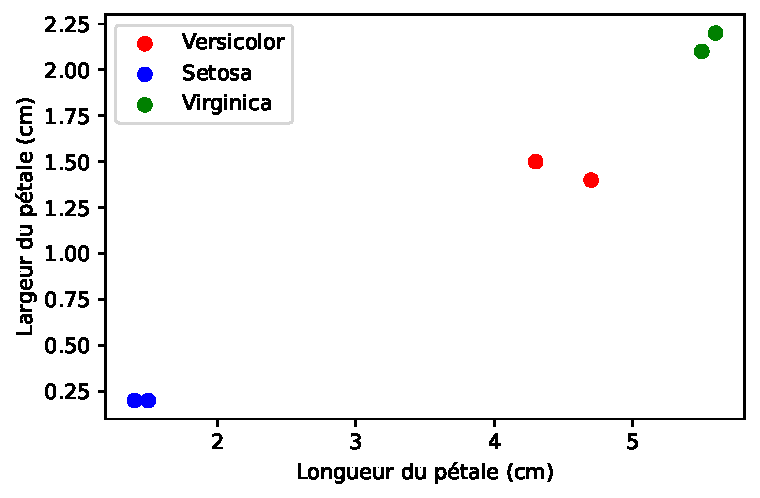
\includegraphics[keepaspectratio]{kppv_cours_files/figure-pdf/cell-2-output-1.pdf}}

Considérons maintenant une fleur d'iris ``Iris X'' dont les pétales ont
une longueur de 3,5 cm et une largeur de 0,75 cm. On souhaite déterminer
la classe de cette fleur.

Ajoutons le point correspondant à ``Iris X'' sur le graphique précédent.

\begin{Shaded}
\begin{Highlighting}[]
\NormalTok{plt.scatter(X[y }\OperatorTok{==} \DecValTok{0}\NormalTok{, }\DecValTok{0}\NormalTok{], X[y }\OperatorTok{==} \DecValTok{0}\NormalTok{, }\DecValTok{1}\NormalTok{], color}\OperatorTok{=}\StringTok{\textquotesingle{}red\textquotesingle{}}\NormalTok{, label}\OperatorTok{=}\StringTok{\textquotesingle{}Versicolor\textquotesingle{}}\NormalTok{)}
\NormalTok{plt.scatter(X[y }\OperatorTok{==} \DecValTok{1}\NormalTok{, }\DecValTok{0}\NormalTok{], X[y }\OperatorTok{==} \DecValTok{1}\NormalTok{, }\DecValTok{1}\NormalTok{], color}\OperatorTok{=}\StringTok{\textquotesingle{}blue\textquotesingle{}}\NormalTok{, label}\OperatorTok{=}\StringTok{\textquotesingle{}Setosa\textquotesingle{}}\NormalTok{)}
\NormalTok{plt.scatter(X[y }\OperatorTok{==} \DecValTok{2}\NormalTok{, }\DecValTok{0}\NormalTok{], X[y }\OperatorTok{==} \DecValTok{2}\NormalTok{, }\DecValTok{1}\NormalTok{], color}\OperatorTok{=}\StringTok{\textquotesingle{}green\textquotesingle{}}\NormalTok{, label}\OperatorTok{=}\StringTok{\textquotesingle{}Virginica\textquotesingle{}}\NormalTok{)}
\NormalTok{plt.scatter(}\FloatTok{3.5}\NormalTok{, }\FloatTok{0.75}\NormalTok{, color}\OperatorTok{=}\StringTok{\textquotesingle{}black\textquotesingle{}}\NormalTok{, label}\OperatorTok{=}\StringTok{\textquotesingle{}Iris X\textquotesingle{}}\NormalTok{)}
\NormalTok{plt.xlabel(}\StringTok{\textquotesingle{}Longueur du pétale (cm)\textquotesingle{}}\NormalTok{)}
\NormalTok{plt.ylabel(}\StringTok{\textquotesingle{}Largeur du pétale (cm)\textquotesingle{}}\NormalTok{)}
\NormalTok{plt.legend()}
\NormalTok{plt.show()}
\end{Highlighting}
\end{Shaded}

\pandocbounded{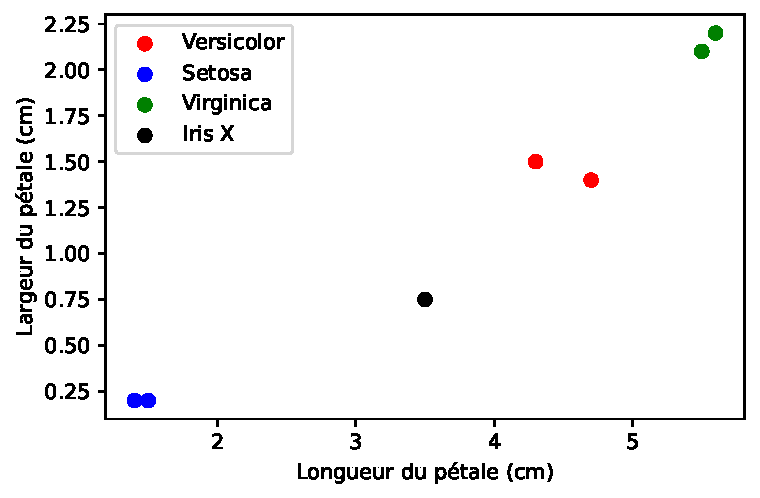
\includegraphics[keepaspectratio]{kppv_cours_files/figure-pdf/cell-3-output-1.pdf}}

Pour déterminer la classe de ``Iris X'', on va calculer la distance
entre ``Iris X'' et chacune des fleurs de l'ensemble E. Nous utilisons
ici la distance euclidienne définie par la formule :

\[AB=\sqrt{(x_B-x_A)^2+(y_B-y_A)^2}\]

pour deux points \(A\) et \(B\) de coordonnées respectivement
\((x_A, y_A)\) et \((x_B, y_B)\) dans un repère orthonormé du plan.

On obtient les résultats suivants :

{\def\LTcaptype{none} % do not increment counter
\begin{longtable}[]{@{}cc@{}}
\toprule\noalign{}
Nom de la fleur & Distance à Iris X (cm) \\
\midrule\noalign{}
\endhead
\bottomrule\noalign{}
\endlastfoot
Iris Setosa 1 & 2.17 \\
Iris Setosa 2 & 2.07 \\
Iris Versicolor 1 & 1.36 \\
Iris Versicolor 2 & 1.10 \\
Iris Virginica 1 & 2.41 \\
Iris Virginica 2 & 2.55 \\
\end{longtable}
}

On décide de donner au paramètre \(k\) la valeur 3. Cela signifie que
l'on cherche les 3 points les plus proches de ``Iris X'' et on détermine
la classe majoritaire parmi ces 3 points.

D'après le tableau ci-dessus, les trois fleurs les plus proches de
``Iris X'' sont ``Iris Versicolor 2'', ``Iris Versicolor 1'' et ``Iris
Setosa 2''. On détermine donc que ``Iris X'' est de la classe
Versicolor.

\textbf{Remarque : en réalité, le nombre d'éléments de l'ensemble E doit
être le plus grand possible pour que l'algorithme soit efficace.}

\begin{tcolorbox}[enhanced jigsaw, arc=.35mm, bottomrule=.15mm, bottomtitle=1mm, breakable, colback=white, colbacktitle=quarto-callout-important-color!10!white, colframe=quarto-callout-important-color-frame, coltitle=black, left=2mm, leftrule=.75mm, opacityback=0, opacitybacktitle=0.6, rightrule=.15mm, title=\textcolor{quarto-callout-important-color}{\faExclamation}\hspace{0.5em}{Important}, titlerule=0mm, toprule=.15mm, toptitle=1mm]

Deux points importants influent sur le résultat de l'algorithme :

\begin{itemize}
\tightlist
\item
  \textbf{Le choix de la distance entre les points} : la distance
  euclidienne n'est pas toujours la meilleure distance possible. Il est
  parfois préférable d'utiliser d'autres distances. On utilise parfois
  la distance Manhattan, définie par : \[AB=|x_B-x_A|+|y_B-y_A|\]
\item
  \textbf{Le choix du nombre de voisins} : le nombre de voisins \(k\)
  doit être suffisamment grand, mais pas trop, pour que l'algorithme
  soit efficace. En général, on choisit une valeur impaire pour éviter
  les cas d'égalité.
\end{itemize}

\end{tcolorbox}

\textbf{Exercice} : les pétales d'un iris ont une longueur de 2,5 cm et
une largeur de 1,25 cm. Déterminer la classe de cette fleur.




\end{document}
